\documentclass[fleqn]{jbook}
\usepackage{physpub}

\begin{document}

\begin{question}{専攻 問題6}{}

図は、レーザー光源を用いたマイケルソン型光干渉計である。Lは周波数の
安定な出力$1\Unit{mW}$のHe-Neレーザー光源(波長$0.63\Unit{\mu m}$)、
P、Qはそれぞれ高い反射率の平面鏡、Sは半透鏡、Dは光検出器(一個の光子が
入ると外部回路に一個の電子を流し得る電流源素子)である。これらは、Sを
除き、それぞれ、干渉信号を得られるように、調整機構を備えた保持具に
取り付けられている。図に示すノブで変位または角度の自由度が調整できる。
また、鏡Pは、モーターMにより、光源の方向に動かせるとする。これらの
保持具は、実験台にネジで固定されており、全体の大きさは$1\Unit{m}$
程度である。光速は$3.0\Keta{8}\Unit{m/s}$、プランク定数$h$は、
$6.6\Keta{-34}\Unit{J\cdot s}$、電子の電荷は、$1.6\Keta{-19}\Unit{C}$
として、以下の設問に答えよ。


\begin{subquestions}
\SubQuestion
  Sで分けられた光が、それぞれP、Qで反射して、再びSで合わさると、干渉
  を起こし、Dには、干渉信号が現れる。干渉信号を得るために、Sに最低限
  必要な調整自由度を持つ保持具を考え、図示せよ。

\SubQuestion
  Dに $50\Unit{\Omega}$の抵抗を接続する。光の強度を強め合う干渉が
  おきている時の抵抗の両端の電圧を評価せよ。また、Pの変位の微小変化に
  対し、出力電圧の変化が最大になるようにPの位置を設定した時、その
  まわりで、Pの位置変化$1\Unit{nm}$に対する出力電圧の変化を評価せよ。

\SubQuestion
  Pがある時刻から急に$10\Unit{m/s^2}$の加速度で外向きに運動し始めた
  とする。Pの速度が$10\Unit{cm/s}$のときの干渉信号は、どのようなもの
  か。また、この干渉信号の時間変化を測定・記録するために考えられる
  測定器・装置を図解し、必要な性能を述べよ。

\SubQuestion
  マイケルソンらは、この種の干渉計(SQ又はSP間の距離約$11\Unit{m}$)を
  静かな地下室に設置して、干渉信号をモニターすることにより、光速度が
  光源の速度に依存しないことを$100$分の$1$程度の精度で示した。その
  原理を簡潔に説明し、この精度を決めている実験的要因を論ぜよ。ただし、
  地球の太陽周りの公転運動の周速度は、約$30\Unit{km/s}$である。

\end{subquestions}
\begin{center}
  \mbox{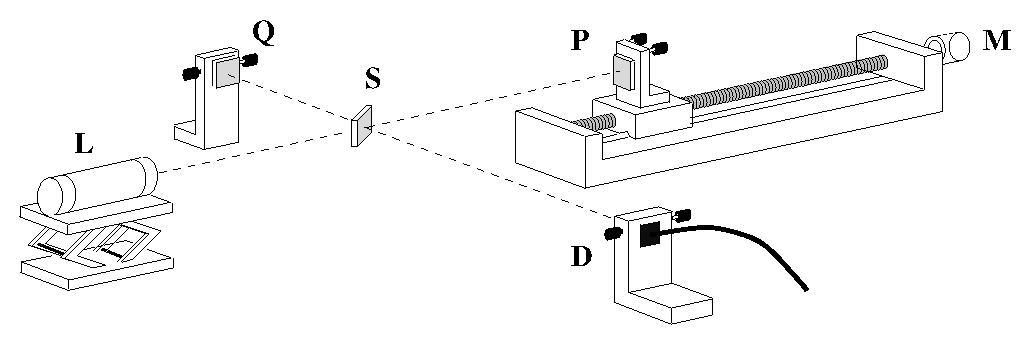
\includegraphics[clip]{1993phy6-1.eps}}
\end{center}

\end{question}
\begin{answer}{専攻 問題6}{}

\begin{subanswers}
  \parbox[t]{105mm}{
\SubAnswer
  半透鏡に必要な自由度は首振り調整と仰角である。右の図の{\bf dial 1}は
  首振り調整用ダイアル、{\bf dial 2}は仰角調整用ダイアルである。

\SubAnswer
  強め合う干渉が起きる時、Dにおける光の強度はほぼレーザーの出力
  に等しい。したがって、出力電圧は
%
  \begin{eqnarray*}
    \lefteqn{({\rm D}に単位時間当たり届く光子の数)%
             \times (電子の電荷) \times (抵抗)} \hspace{10mm}\\
    &=& \frac{1\Unit{mW}}{hc/\lambda}%
        \times e \times 50\Unit{\Omega}%
     =  2.5\Keta{-2}\Unit{V} \hspace{5mm}% 
        ( \, \equiv \, V_{\rm max} )
  \end{eqnarray*}
%
  また、Pの位置を $\IDelta L$ だけ変化させた時の出力電圧は、
  適当な位相因子を除いて、
%
  \[ V_{\rm max}\cos^{2}\left(\frac{2\pi\IDelta L}{\lambda}\right)%
     = \frac{1}{2} V_{\rm max} \left\{ 1 + \cos%
       \left( \frac{4\pi \IDelta L}{\lambda} \right) \right\} \]
%
  と書ける。すると、出力電圧の変化が最大になるのは
  }\parbox[t]{50mm}{
  \begin{center}
    \mbox{\includegraphics[clip]{1993phy6-2.eps}}
  \end{center}}
%
  \[ \Deriver{}{(\IDelta L)} \frac{1}{2} V_{\rm max} 
     \left\{ 1 + \cos \left( \frac{4\pi \IDelta L}{\lambda} \right) 
     \right\} = \frac{2\pi}{\lambda} V_{\rm max}
     \sin \left( \frac{4\pi \IDelta L}{\lambda} \right) = 0%
     \hspace{10mm}%
     \frac{\IDelta L}{\lambda} = \frac{1}{2},1,\frac{3}{2},\cdots \]
%
  の時である。この時の出力電圧の変化率は、明らかに
  $ V_{\rm max} \times 2\pi/\lambda $である。

  このまわりで、Pが$1\Unit{nm}$だけずれると、出力電圧は
%
  \[ V_{\rm max} \times \frac{2\pi}{\lambda} 
     \times 1\Unit{nm} = 2.5\Keta{-4} \Unit{V} \]
%
  だけ変化する。 



\SubAnswer
  SとPの距離を$x(t)$とする($t$は時刻)。今、装置の大きさが充分小さく、
  Pの速度も小さい。時刻$t$にSを出た光がPで反射し再びSに時刻$t'$に
  戻ったとすると、
%
  \[ t' \simeq t + \frac{2x(t)}{c} \hspace{10mm}%
     \d{t}' = \d{t}+\frac{2\dot{x}(t)}{c}\d{t} \]
%
  したがって、レーザーの角周波数を$\omega_{0}$とすると、Pで反射した
  光の角周波数は
%
  \[ \omega = \frac{1}{1+2\dot{x}/c} \omega_{0} \simeq%
              \left(1-\frac{2\dot{x}}{c} \right) \omega_{0} \]
%
  となる。よってDにおける干渉信号は、
%
  \[ \cos \omega t + \cos \omega_{0} t%
       = 2\cos{\left(\frac{\omega-\omega_{0}}{2}t\right)}%
          \cos{\left(\frac{\omega+\omega_{0}}{2}t\right)}%
  \simeq 2\cos{\left(\frac{\dot{x}}{c}\omega_{0}t\right)}%
          \cos{\omega_{0}t} \]
%
  より、$\cos{(\frac{\dot{x}}{c}\omega_{0}t)}$のように変化する。\\
%
  可視光領域であるから測定できるのは $\cos{\omega_0 t}$ の振幅の
  2乗である。$\dot{x}=10\Unit{cm/s}$の時のその値は、
%
  \[ 2 \times \frac{\dot{x}}{c} \times \frac{c}{\lambda}%
     = 3\Keta{5} \Unit{Hz} \]
%
  で振動する。これを記録するには次ページの図のような装置を組めばよい。
%
  \begin{center}
    \mbox{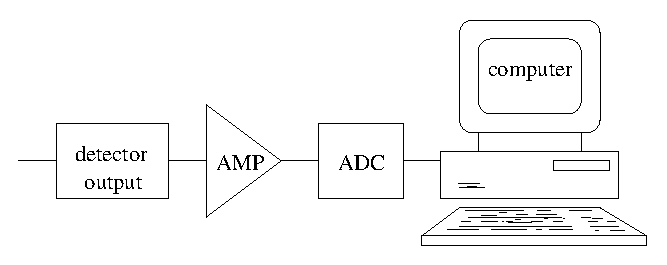
\includegraphics[clip]{1993phy6-3.eps}}
  \end{center}
%
  ただしアンプは$10^3\sim 10^6\Unit{Hz}$程度の周波数に応答できるものを使う。


\SubAnswer
  マイケルソン--モーレーの実験ではDに生ずる干渉縞を観測する。
  まず、SP=SQ=$l$とし、SPを地球の公転方向に向ける。
  ここで、いわゆる「エーテルの風」があるとすると、
  SP往復に要する時間は公転速度を$v$として、
%
  \[ t_{1} = \frac{l}{c-v} + \frac{l}{c+v}%
     \simeq \frac{l}{c}\left(1+\frac{v}{c}+\frac{v^2}{c^2}\right)%
     + \frac{l}{c} \left( 1 - \frac{v}{c} + \frac{v^2}{c^2} \right)%
     = \frac{2l}{c}\left(1+\frac{v^2}{c^2}\right) \]
%
  SQ往復に要する時間は
%
  \[ t_{2} = \frac{2l}{\sqrt{c^2-v^2}}%
     \simeq \frac{2l}{c}\left(1-\frac{v^2}{c^2}\right)^{-\frac{1}{2}}%
     = \frac{2l}{c} \left( 1+\frac{v^2}{2c^2} \right) \]
%
  したがって、$t_{1}-t_{2}=lv^2/c^3$ となる。

  次に、装置を$90\deg$回転して同じことを行なうと、明らかに
  $t_{1}-t_{2}=-lv^2/c^3$となる。したがって、Dで観測される干渉縞は
  $2c(t_{1}-t_{2})=2lv^2/c^2$だけずれるはずである。このずれを波長に
  直すと、
%
  \[  \frac{2lv^2/c^2}{\lambda}%
    = \frac{2\times 11\Unit{m}}{0.63\Unit{\mu m}}%
      \left( \frac{3.0\Keta{4}\Unit{m/s}}{3.0\Keta{8}\Unit{m/s}}%
      \right)^{2} \sim 0.3 \]
%
  となる。「エーテルの風」がない場合、つまり光速度が光源の速度に
  依らない場合はこのずれは観測されない。これが、マイケルソン--モーレー
  の実験の原理である。\\
%
  実験の精度はSP、SQの距離が本当に一定に保たれているかに大きく依って
  いる。したがって、温度変化や装置の振動による器具のゆがみに影響を
  受ける。また、光線にはある程度広がりがあるので、干渉縞の位置にも
  誤差が含まれる。

\end{subanswers}
\end{answer}


\end{document}
